% Desenvolvido por:
% Clodoaldo de Souza Faria Júnior - Aluno Engenharia Elétrica
% Leonardo Ataide Carniato - Professor Engenharia Elétrica
% Versão: 09/02/2022

\documentclass[
	% -- opções da classe memoir --
	12pt,				% tamanho da fonte
	openright,			% capítulos começam em pág ímpar (insere página vazia caso preciso)
	oneside,			% para impressão em verso e anverso.  Usar twoside
	a4paper,			% tamanho do papel. 
	%normalfigtabnum,
	%pnumromarab,
	% -- opções da classe abntex2 --
	chapter=Title,		% títulos de capítulos convertidos em letras maiúsculas
	%section=TITLE,		% títulos de seções convertidos em letras maiúsculas
	%subsection=TITLE,	% títulos de subseções convertidos em letras maiúsculas
	%subsubsection=TITLE,% títulos de subsubseções convertidos em letras maiúsculas
	% -- opções do pacote babel --
	english,			% idioma adicional para hifenização
	french,				% idioma adicional para hifenização
	spanish,			% idioma adicional para hifenização
	brazil,				% o último idioma é o principal do documento
]{abntex2}

\setlrmarginsandblock{3cm}{2cm}{*}
\setulmarginsandblock{3cm}{2cm}{*}
\checkandfixthelayout


% ---------------------------------------------------------------------------------
%                                   PACOTES
% ---------------------------------------------------------------------------------

% ---
% Pacotes básicos 
% ---
\usepackage{mathptmx}			% Usa a fonte Times New Roman
\usepackage[T1]{fontenc}		% Selecao de codigos de fonte.
\usepackage{lastpage}			% Usado pela Ficha catalográfica
\usepackage{indentfirst}		% Indenta o primeiro parágrafo de cada seção.
\usepackage{xcolor,colortbl}	% Controle das cores
\usepackage{graphicx}			% Inclusão de gráficos
\usepackage{microtype} 			% para melhorias de justificação
\usepackage{hyperref}
\usepackage{subfig}
\usepackage{epigraph}
\usepackage{url}
\usepackage{placeins}
\newcommand*{\rom}[1]{\expandafter\@slowromancap\romannumeral #1@}
\usepackage{multirow}
\usepackage[figuresright]{rotating}
\usepackage{chemfig}
\usepackage{amsmath}
\usepackage{amssymb}
\usepackage{enumitem}
\usepackage{bigints}
\usepackage{listings}
\usepackage{etoolbox}
\usepackage[final]{pdfpages}
\usepackage{bigstrut}
\usepackage{mathtools}
\usepackage{gensymb}
\usepackage{epsfig}
\usepackage{booktabs}
\usepackage{longtable}
\usepackage[bottom]{footmisc}
\usepackage{float}
\DeclareUnicodeCharacter{00A0}{ }
\renewcommand{\sfdefault}{\rmdefault}

% ---
% Pacotes adicionais, usados apenas no âmbito do Modelo Canônico do abnteX2
% ---
\usepackage{lipsum}				% para geração de dummy text
% ---

% ---
% Pacotes de citações
% ---
\usepackage[brazilian,hyperpageref]{backref}	 % Paginas com as citações na bibl
\usepackage[alf,abnt-emphasize=bf,abnt-etal-text=emph,bibjustif]{abntex2cite}  % Citações padrão ABNT


% ---------------------------------------------------------------------------------
%                          CONFIGURAÇÕES DOS PACOTES
% ---------------------------------------------------------------------------------

% ---
% Configurações do pacote backref
%
% Para desativar, tire o comentário de \begin{comment} e \end{comment} 
% das próximas linhas e comente a linha \usepackage[brazilian,hyperpageref]{backref}
% acima.
% ---

%\begin{comment}
% ---
% Configurações do pacote backref
% Usado sem a opção hyperpageref de backref
\renewcommand{\backrefpagesname}{Citado na(s) página(s):~}
% Texto padrão antes do número das páginas
\renewcommand{\backref}{}
% Define os textos da citação
\renewcommand*{\backrefalt}[4]{
	\ifcase #1 %
	Nenhuma citação no texto.%
	\or
	Citado na página #2.%
	\else
	Citado #1 vezes nas páginas #2.%
	\fi}%
% ---
%\end{comment}


% listagens
\definecolor{corComentario}{RGB}{150,150,150}
\definecolor{corString}{RGB}{206,123,0}
\definecolor{corPalavraChave}{RGB}{0,0,230}

\lstset{
	numbers=left,
	stepnumber=1,
	firstnumber=1,
	numberstyle=\footnotesize,
	extendedchars=true,
	breaklines=true,
	lineskip=0pt,
	frame=tb,
	basicstyle=\ttfamily\footnotesize,
	showstringspaces=false,
	stringstyle=\color{corString},
	commentstyle=\color{corComentario},
	keywordstyle=\color{corPalavraChave}
}

\newcolumntype{Y}{>{\centering\arraybackslash}X}

\newcommand{\ano}[1]{\def \oano {#1}}
\newcommand{\imprimirano}{\oano}

\newcommand{\mes}[1]{\def \omes {#1}}
\newcommand{\imprimirmes}{\omes}

\newcommand{\subtitulo}[1]{\def \osubtitulo {#1}}
\newcommand{\imprimirsubtitulo}{\osubtitulo}

\newcommand{\area}[1]{\def \aarea {#1}}
\newcommand{\imprimirarea}{\aarea}

\renewcommand{\coorientador}[1]{\def \ocoorientador {#1}}
\renewcommand{\imprimircoorientador}{\ocoorientador}

\newcommand{\grau}[1]{\def \ograu {#1}}
\newcommand{\imprimirgrau}{\ograu}

\newcommand{\curso}[1]{\def \ocurso {#1}}
\newcommand{\imprimircurso}{\ocurso}


% ---
% Informações de dados para CAPA e FOLHA DE ROSTO
% ---

\curso{Bacharelado em Engenharia Elétrica}
\grau{Bacharel em Engenharia Elétrica}

\titulo{Título}

% caso não haja subtítulo, comente a linha abaixo
\subtitulo{Subtítulo}

\tipotrabalho{Trabalho de Conclusão de Curso}
\area{Área}

\autor{Autor}
\orientador{Orientador}

% caso não haja coorientador, comente a linha abaixo
\coorientador{Coorientador}

\local{Presidente Epitácio}
\mes{Mês}
\ano{2022}

\instituicao{%
	Instituto Federal de Educação, Ciência e Tecnologia de São Paulo - Câmpus Presidente Epitácio
	\par
	Curso bacharelado em Engenharia Elétrica
}

\preambulo{\imprimirtipotrabalho\ apresentado ao Curso de Bacharelado em Engenharia Elétrica do Instituto Federal de Educação, Ciência e Tecnologia de São Paulo - Câmpus Presidente Epitácio, como parte dos requisitos para obtenção grau de \imprimirgrau.
}
% ---


% ---
% Configurações de aparência do PDF final
% ---

% alterando o aspecto da cor azul
\definecolor{blue}{RGB}{41,5,195}

% informações do PDF
\makeatletter
\hypersetup{
	%pagebackref=true,
	pdftitle={\@title}, 
	pdfauthor={\@author},
	pdfsubject={\imprimirpreambulo},
	pdfcreator={Nome Completo},
	pdfkeywords={Palavra chave 1}{Palavra chave 2}{Palavra chave 3}{Palavra chave n}, 
	colorlinks=true,       		% false: boxed links; true: colored links
	linkcolor=black,          	% color of internal links
	citecolor=black,       		% color of links to bibliography
	filecolor=black,      		% color of file links
	urlcolor=black,
	bookmarksdepth=4
}
\makeatother
% --- 
% ---
% Comandos do autor
% ---

% comando para inserir autor e ano
\newcommand{\citeauthorandyear}[1]{\citeauthoronline{#1} (\citeyear{#1})}


% ---
% Novo list of (listings) para Quadros
% ---



% configurações para atender às regras da ABNT
\setfloatadjustment{quadro}{\centering}
%\counterwithout{quadro}{chapter}
%\renewcommand{\cftquadroname}{\quadroname\space} 
%\renewcommand*{\cftquadroaftersnum}{\hfill--\hfill}

% Configuração de posicionamento padrão:
\setfloatlocations{quadro}{hbtp}



% --- 
% Espaçamentos entre linhas e parágrafos 
% --- 

% O tamanho do parágrafo é dado por:
\setlength{\parindent}{1.3cm}

% Controle do espaçamento entre um parágrafo e outro:
\setlength{\parskip}{0.2cm}  % tente também \onelineskip

% ---
% compila o indice
% ---
\makeindex
% ---







% ---------------------------------------------------------------------------------
%                                   INÍCIO DO DOCUMENTO
% ---------------------------------------------------------------------------------
\begin{document}
\newcommand{\quadroname}{Quadro}
\newcommand{\listofquadrosname}{\normalsize \bfseries LISTA DE QUADROS}
\renewcommand{\listadesimbolosname}{\normalsize \bfseries  LISTA DE SÍMBOLOS}
\renewcommand{\listadesiglasname}{\normalsize \bfseries LISTA DE ABREVIATURAS E SIGLAS}
\renewcommand{\agradecimentosname}{\normalsize \bfseries AGRADECIMENTOS}
\renewcommand{\resumoname}{\normalsize \bfseries RESUMO}
\addto\captionsbrazil{\renewcommand{\listfigurename}{\normalsize \bfseries LISTA DE FIGURAS}}
\addto\captionsbrazil{\renewcommand{\listtablename}{\normalsize \bfseries LISTA DE TABELAS}}
\addto\captionsbrazil{\renewcommand{\bibname}{\normalsize \bfseries REFERÊNCIAS}}
\addto\captionsbrazil{\renewcommand{\contentsname}{\normalsize \bfseries SUMÁRIO}}

% Seleciona o idioma do documento (conforme pacotes do babel)
%
% Retira espaço extra obsoleto entre as frases.

\selectlanguage{brazil}
\frenchspacing 




% ---------------------------------------------------------------------------------
%                                   ELEMENTOS PRÉ-TEXTUAIS
% ---------------------------------------------------------------------------------
%\pretextual

% ---
% Capa
% ---
%\imprimircapa
% capa personalizada

\begin{center}
	
	\center
	
\includegraphics[width=0.3\textwidth]{_logoifsp.jpg}
	\vspace{0.5cm}
	\\
	\ABNTEXchapterfont\textsc{\textbf{\MakeUppercase{\imprimirinstituicao}}}
	\vspace{3.5cm}
	
    \ABNTEXchapterfont\textsc{\MakeUppercase{\textbf{\imprimirautor}}}
	\vspace{3.5cm}
	
    \ABNTEXchapterfont\textsc{\MakeUppercase{\textbf{\imprimirtitulo\ifdef{\osubtitulo}{:}{}}}}
    
    \ifdef{\osubtitulo}{\MakeUppercase{\ABNTEXchapterfont\imprimirsubtitulo}}{}
	\vfill
	
	\textsc{\MakeUppercase{\textbf{\imprimirlocal}}}
	
	\textsc{\MakeUppercase{\textbf{\imprimirano}}}
	
	\vspace*{2cm}
	
\end{center}

\cleardoublepage


% ---

% ---
% Folha de rosto
% (o * indica que haverá a ficha bibliográfica)
% ---
%\imprimirfolhaderosto*
\begin{center}
   	
   	\ABNTEXchapterfont\textsc{\MakeUppercase{\textbf{\imprimirautor}}}
   	\vspace{2.5cm}
   	
    \ABNTEXchapterfont\textsc{\MakeUppercase{\textbf{\imprimirtitulo\ifdef{\osubtitulo}{:}{}}}}
                           
    \ifdef{\osubtitulo}{\MakeUppercase{\ABNTEXchapterfont\imprimirsubtitulo}}{}
   	\vspace{2.5cm}
   	   	
   	\hspace{.42\textwidth}
   	\begin{minipage}{.55\textwidth}
   		\SingleSpacing
   		\small\imprimirpreambulo
   		
   		\vspace{\onelineskip}
   	
   		
   	\end{minipage}%
   		\center
        \normalsize
   		Orientador: \imprimirorientador
   		
        \ifdef{\ocoorientador}{
     		\vspace{\onelineskip}
   		
    		Coorientador: \imprimircoorientador
        }{}
    \vfill
   	
	\textsc{\MakeUppercase{\textbf{\imprimirlocal}}}
	
	\textsc{\MakeUppercase{\textbf{\imprimirano}}}
   	
   	\vspace*{2cm}
   	
\end{center}


% ---

% ---
% Inserir a ficha catalográfica
% ---
%
% Este é um exemplo de ficha catalográfica.
%
% A ficha catalográfica final deve ser requisitada pelo aluno e inserida neste
% documento para a entrega da versão final.
%

\begin{fichacatalografica}
    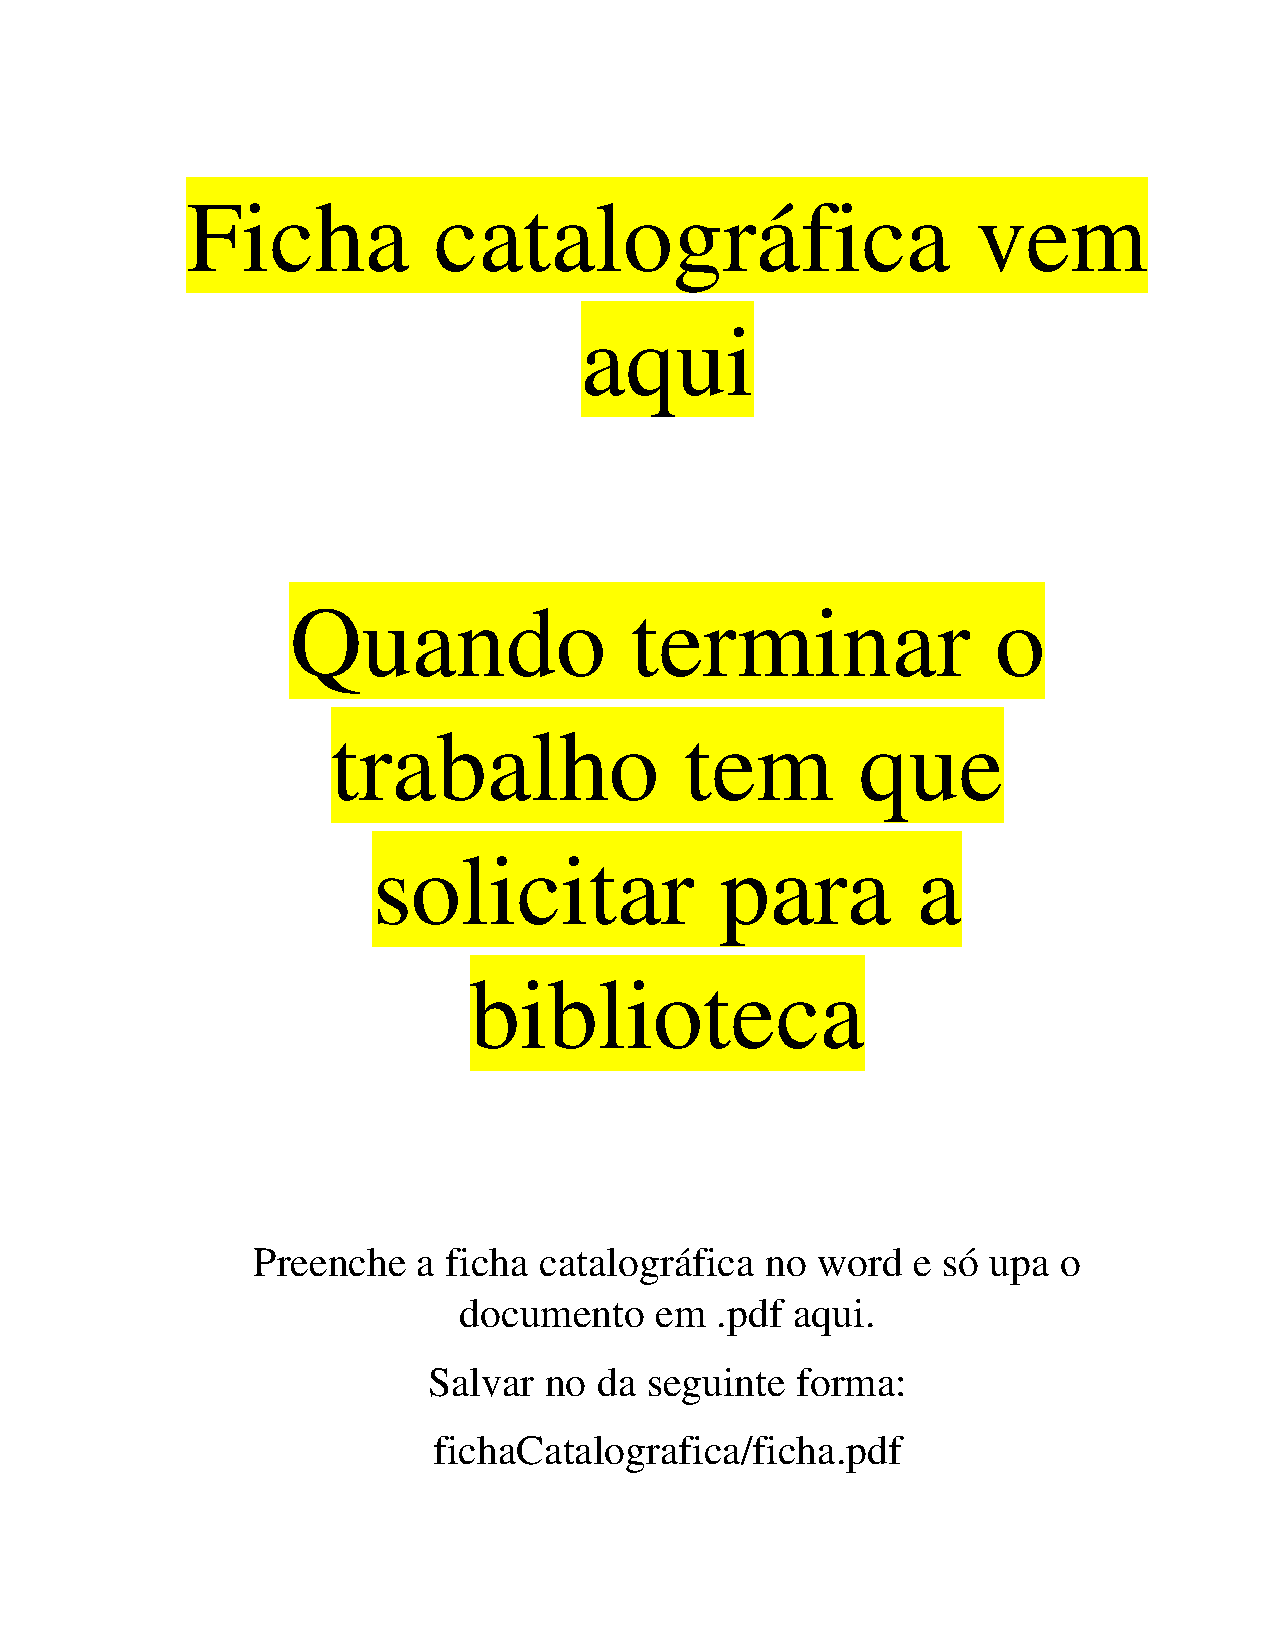
\includepdf{fichaCatalografica/ficha.pdf}
\end{fichacatalografica}

% ---
% Inserir folha de aprovação
% ---
%
% Este é um exemplo de folha de aprovação.
%
% A folha de aprovação final será inserida pelo Coordenador do Curso.
%

\begin{folhadeaprovacao}
	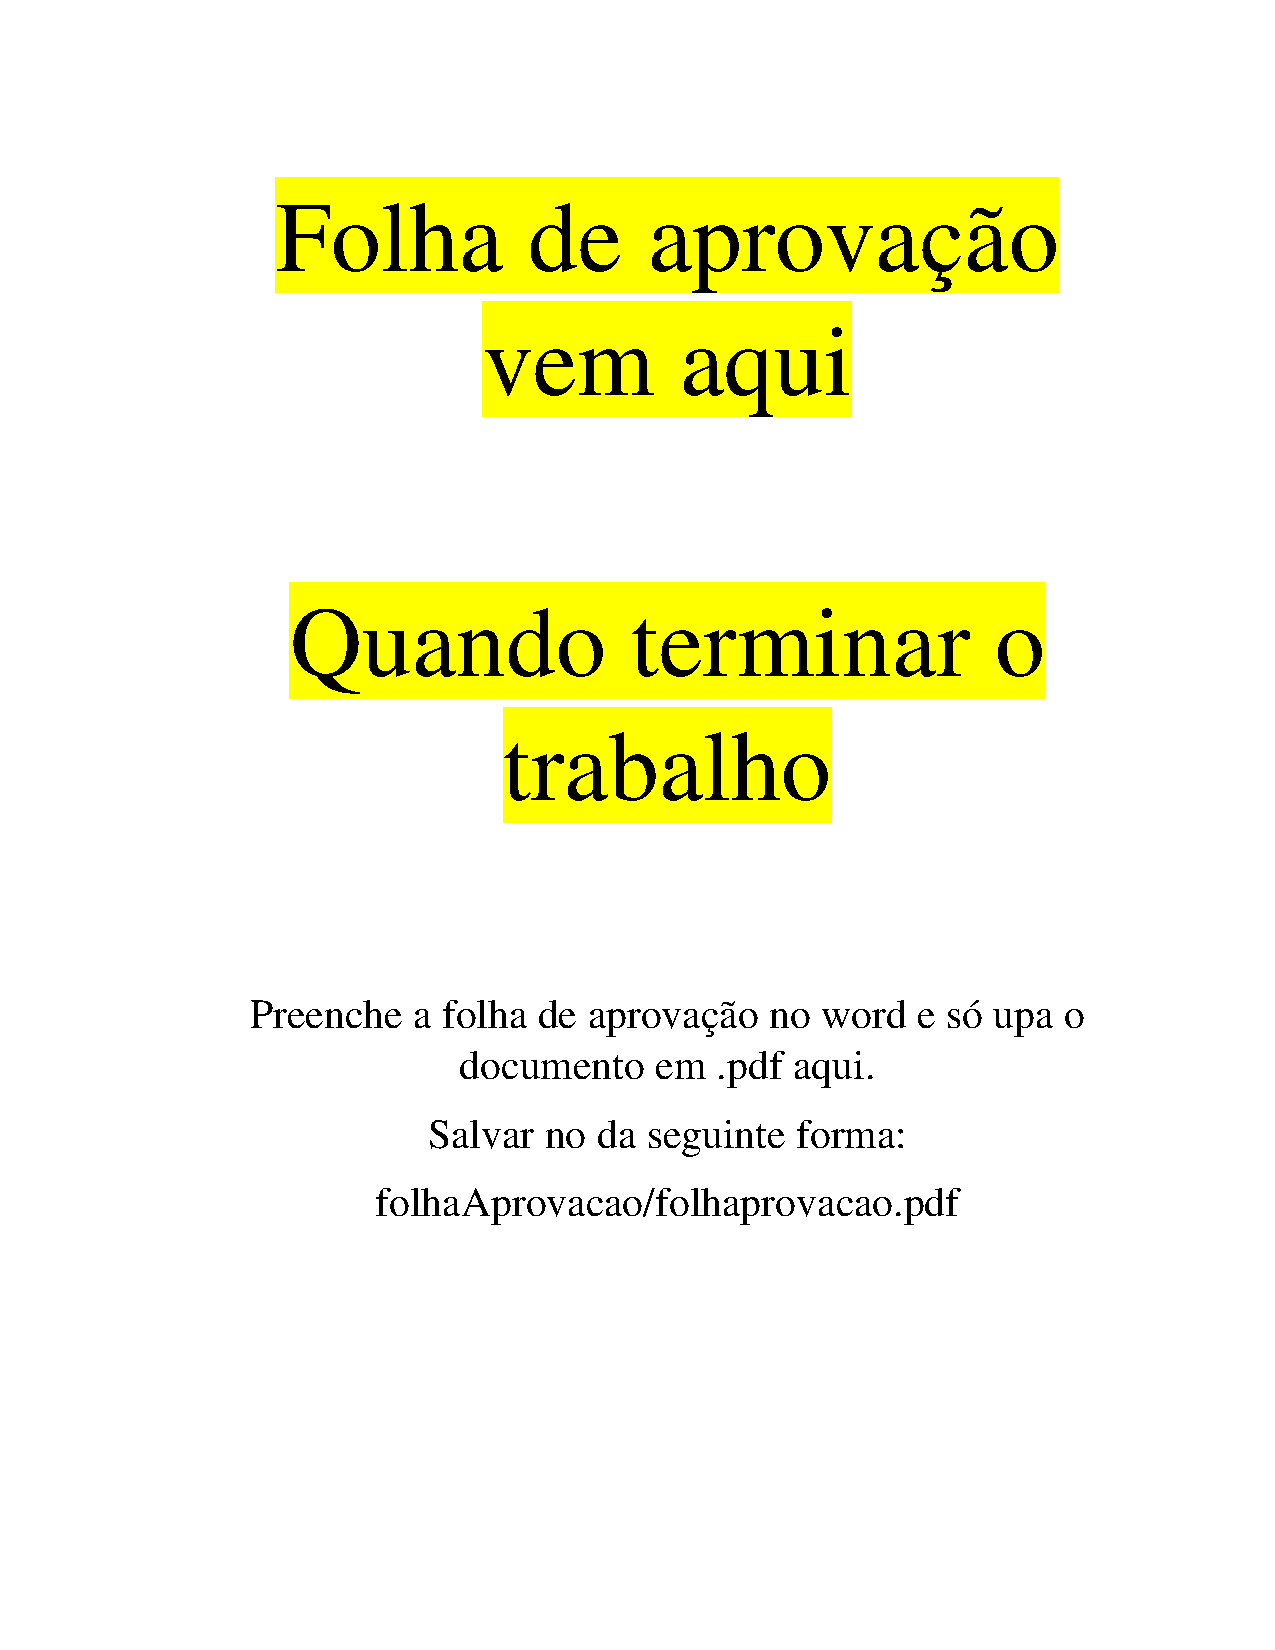
\includepdf{folhaAprovacao/folhaprovacao.pdf}
\end{folhadeaprovacao}

% ---
% Dedicatória
% ---
%\begin{dedicatoria}
	\vspace*{\fill}
	\centering
	\noindent
	\textit{Dedicatória (Opcional). Não digite a palavra Dedicatória. Texto no qual o autor do trabalho oferece homenagem ou dedica o seu trabalho a alguém (não usar ponto final)}
    \vspace*{\fill}
\end{dedicatoria}

% ---
% Agradecimentos
% ---
\begin{agradecimentos}

Gostaria de agradecer...
	
\end{agradecimentos}

% ---
% Epígrafe
% ---
%\begin{epigrafe}
	
	\vspace*{\fill}
	Epígrafe (Opcional). Pensamentos retirados de um livro, uma música, um poema, normalmente relacionado ao tema do trabalho, seguida de indicação de autoria. As epígrafes podem ser colocadas também nas folhas de abertura de cada capítulo.  
    
	\epigraph{``\emph{Any fool can write code that a computer can understand. Good programmers write code that humans can understand}''.}{Martin Fowler}
	
\end{epigrafe}

% ---
% Resumos
% ---
\setlength{\absparsep}{18pt} % ajusta o espaçamento dos parágrafos do resumo
\begin{resumo}
	
	Resumo
	
	\vspace{\onelineskip}
	
	\textbf{Palavras-chave}: 1. Palavra-chave  2. Palavra-chave 3. Palavra-chave.
	
\end{resumo}

\setlength{\absparsep}{18pt} % ajusta o espaçamento dos parágrafos do resumo
\begin{resumo}[\normalsize \bfseries ABSTRACT]
	
	\begin{otherlanguage*}{english}
		
		Abstract
		
		\vspace{\onelineskip}
		 
		\textbf{Keywords}: 1. Keyword 2. Keyword 3. Keyword.
		
	\end{otherlanguage*}

\end{resumo} 

% ---
% inserir lista de ilustrações
% ---
\pdfbookmark[0]{\listfigurename}{Lista de Figuras}
\listoffigures*
\cleardoublepage
% ---

% ---
% inserir lista de quadros
% ---
%\pdfbookmark[0]{\listofquadrosname}{loq}
%\listofquadros*
%\cleardoublepage
% ---

% ---
% inserir lista de tabelas
% ---
%\pdfbookmark[0]{\listtablename}{lot}
\listoftables*
\cleardoublepage
% ---

% ---
% inserir lista de abreviaturas e siglas
% ---
\begin{siglas}
    \item[CDDIS] \textit{Crustal Dynamics Data Information System}
\end{siglas}
% ---

% ---
% inserir lista de símbolos
% ---
\begin{simbolos}
	\item[$f_o$] Frequência fundamental
\end{simbolos}
% ---

% ---
% inserir o sumário
% ---
%\pdfbookmark[0]{\contentsname}{toc}
\tableofcontents*
\cleardoublepage
% ---


% ---------------------------------------------------------------------------------
%                                  ELEMENTOS TEXTUAIS
% ---------------------------------------------------------------------------------
\textual
\renewcommand{\ABNTEXchapterfont}{\rmfamily\bfseries\MakeUppercase}
\renewcommand{\ABNTEXchapterfontsize}{\normalsize}
\renewcommand{\ABNTEXsectionfont}{\ABNTEXchapterfont}
\renewcommand{\ABNTEXsectionfontsize}{\normalsize}
\renewcommand{\ABNTEXsubsectionfont}{\ABNTEXsectionfont}
\renewcommand{\ABNTEXsubsectionfontsize}{\normalsize}
\renewcommand{\ABNTEXsubsubsectionfont}{\ABNTEXsubsectionfont}
\renewcommand{\ABNTEXsubsubsectionfontsize}{\normalsize}
\renewcommand{\tocheadstart}{\ABNTEXchapterfont}







\chapter{INTRODUÇÃO}
\label{cap:01}

Introdução
\chapter{REVISÃO DA LITERATURA}
\label{cap:02}

Revisão da literatura
\chapter{METODOLOGIA}
\label{cap:03}

Metodologia
\chapter{RESULTADOS E DISCUSSÃO}
\label{cap:04}

Resultados
\chapter{CONCLUSÕES}
\label{cap:05}

Conclusões
%\chapter{Cronograma}
\label{cap:06}

Segue abaixo o cronograma das atividades que serão executadas até a Avaliação Final de TCC.

\textbf{Obs:} Para facilitar, crie o cronograma usando o modelo do Word contido no projeto (imagens/templateCronograma.docx), ou qualquer outro \textit{software}, salve a imagem e atualize o arquivo imagens/cronograma.png.

\FloatBarrier
\begin{figure*}[!htbp]
	\centering
	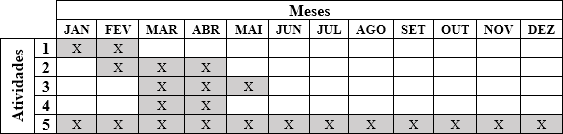
\includegraphics[scale=1]{imagens/cronograma}
\end{figure*}
\FloatBarrier

\begin{enumerate}
	\item Descrição da atividade 1;
	\item Descrição da atividade 2;
	\item Descrição da atividade 3;
	\item Descrição da atividade 4;
	\item Descrição da atividade 5.
\end{enumerate}

\textbf{Obs:} Este capítulo deve ser elaborado e estar contido em trabalhos de graduação para a Validação de Projeto de TCC. Na Avaliação Final de TCC este capítulo não deve existir, visto que não haverá atividades após a Avaliação Final.





% ---------------------------------------------------------------------------------
%                                 ELEMENTOS PÓS-TEXTUAIS
% ---------------------------------------------------------------------------------
\postextual


% ----------------------------------------------------------
% Referências bibliográficas
% ----------------------------------------------------------
\bibliography{referencias}

% ----------------------------------------------------------
% Glossário
% ----------------------------------------------------------
%
% Consulte o manual da classe abntex2 para orientações sobre o glossário.
%
%\glossary


% ----------------------------------------------------------
% Apêndices
% ----------------------------------------------------------
%% Texto ou documento elaborado pelo autor, a fim de complementar sua argumentação, sem prejuízo da unidade nuclear do trabalho.

% ---
% Inicia os apêndices
% ---
\begin{apendicesenv}
	
	% Imprime uma página indicando o início dos apêndices
	\partapendices
	
	% ----------------------------------------------------------
	\chapter{Título do Apêndice A}
	% ----------------------------------------------------------
	
	Texto do Apêndice A.
	
	
	
	% ----------------------------------------------------------
	\chapter{Título do Apêndice B}
	% ----------------------------------------------------------
	
	Texto do Apêndice B.
	
	
	
	% ----------------------------------------------------------
	\chapter{Título do Apêndice C}
	% ----------------------------------------------------------
	
	Texto do Apêndice C.
	
	
	
	% ----------------------------------------------------------
	\chapter{Título do Apêndice D}
	% ----------------------------------------------------------
	
	Texto do Apêndice D.
	
	
	
	% ----------------------------------------------------------
	\chapter{Título do Apêndice E}
	% ----------------------------------------------------------
	
	Texto do Apêndice E.
	
	
	
\end{apendicesenv}
% ---


% ----------------------------------------------------------
% Anexos
% ----------------------------------------------------------
%% Texto ou documento não elaborado pelo autor, que serve de fundamentação, comprovação e ilustração.

% ---
% Inicia os anexos
% ---
\begin{anexosenv}
	
	% Imprime uma página indicando o início dos anexos
	\partanexos
	
	% ----------------------------------------------------------
	\chapter{Título do Anexo A}
	% ----------------------------------------------------------
	
	Texto do Anexo A.
	
	
	
	% ----------------------------------------------------------
	\chapter{Título do Anexo B}
	% ----------------------------------------------------------
	
	Texto do Anexo B.
	
	
	
	% ----------------------------------------------------------
	\chapter{Título do Anexo C}
	% ----------------------------------------------------------
	
	Texto do Anexo C.
	
	
	
	% ----------------------------------------------------------
	\chapter{Título do Anexo D}
	% ----------------------------------------------------------
	
	Texto do Anexo D.
	
	
	
	% ----------------------------------------------------------
	\chapter{Título do Anexo E}
	% ----------------------------------------------------------
	
	Texto do Anexo E.
	
	
	
\end{anexosenv}


%---------------------------------------------------------------------
% ÍNDICE REMISSIVO
%---------------------------------------------------------------------

%\phantompart

%\printindex

\newlistof{listofquadros}{loq}{\listofquadrosname}
\newlistentry{quadro}{loq}{0}

\end{document}
